
\section*{Introducción}
Los amplificadores operacionales (op-amps) son dispositivos electrónicos fundamentales en el diseño de circuitos analógicos, ya que permiten amplificar señales muy pequeñas, realizar operaciones matemáticas y procesar información en función a una configuración entre sus entradas, siendo así que para tal propósito es necesario contar con cierta precisión entre su terminales diferenciales, por lo tanto un análisis de las corrientes de polarización es necesario para lograr este objetivo el cual afecta a mediciones de rango pequeño como las provenientes del cuerpo humano o en la industrial en las cuales los requisitos de voltaje y/o corriente son pequeños para extender el tiempo de vida de un determinado sensor.

Así mismo dentro del desarrollo de esta experiencia se verá en pleno funcionamiento de 2 amplificadores operacionales y su respuesta y/o tensión de offset y corrientes de bias (polarización) entre sus entradas inversora y no inversora, para lo cu	al se emplea un circuito de prueba.


\section{ Mediciones de voltaje divisor de tensión y amplificadores operacionales}

Como punto de partida se compararon los niveles de voltaje obtenidos a partir de un divisor de tensión utilizando el mismo circuito en un etapa posterior para la medición del voltaje obtenido previamente mediante los operacionales LM741 y el TL081 en una configuración de seguidor de voltaje, en la figura \ref{fig:divisor-tension} la configuración inicial y en la figura \ref{fig:seguidor-tension} la configuración para los operacionales anteriormente mencionados.

\begin{figure}[h]
	\centering
	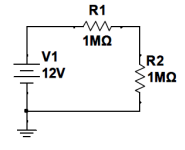
\includegraphics[width=0.3\linewidth]{media/divisor-tension}
	\caption{Medición de voltaje - divisor de tensión}
	\label{fig:divisor-tension}
\end{figure}

% TODO: \usepackage{graphicx} required
\begin{figure}[h]
	\centering
	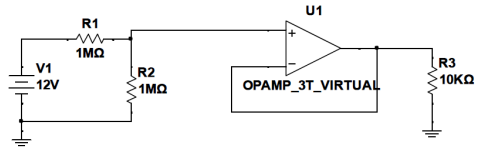
\includegraphics[width=0.8\linewidth]{media/seguidor-tension}
	\caption{Seguidor de tensión}
	\label{fig:seguidor-tension}
\end{figure}

Las mediciones para cada circuito con el operacional indicado se muestran en la tabla \ref{tab:mediciones-voltaje} y de la cual se puede inferir que existen una cierta variación entre los valores esperados idealmente según las consideraciones teóricas para los amplificadores operacionales, lo que destaca en cierta forma la existencia de un fenómeno electrico no considera dentro del análisis general usado para el estudio de los operacionales.

\begin{table}[]
	\centering
	\begin{tabular}{|l|l|}
		\hline
		& Voltaje {[}V{]} \\ \hline
		R2    & 5.61            \\ \hline
		LM741 & 5.88            \\ \hline
		TL081 & 5.9             \\ \hline
	\end{tabular}
	\caption{Mediciones de voltaje}
	\label{tab:mediciones-voltaje}
\end{table}

\subsection{Voltaje medido y esperado}
Debido a las diferencias de voltaje para componente usado en la experiencia este de forma teórica se debido aproximar al voltaje medido en la resistencia $R_2$ y el cual se esperaba verse reflejado en la resistencia $R_3$, sin embargo y como se verá más adelante la diferencia entre estos valores de salida ocurre a un desbalance en la entrada de cada operacional y que se conoce como los valores offset el amp. operacional y que se debe tener en cuenta para aplicaciones que requieran de pequeñas variaciones en las salidas.

\section{Medición $V_O$ y cálculo de $V_{OS}$ }

Las mediciones realizadas durante la experiencia se realizaron en el circuito mostrado en la figura \ref{fig:opam-offset} y con el cual bajo las consideraciones indicadas $R_4$ y $R_5$ cortocircuitadas, se realizo la medición del voltaje de salida $V_O$ y en función a ello se determino el valor de $V_{OS}$ en función a la relación indicada en \ref{eq:vos-calculo}.

\begin{equation}
	V_{OS} = -\frac{V_O}{1 + \frac{R_6}{100}}
	\label{eq:vos-calculo}
\end{equation}

Obteniendo como medición y resultado para cada operacional los datos mostrados en la tabla \ref{tab:mediciones-vo-vos} denotándose una pequeña variación en las tensiones de salida que rondan tan solo las milésima y con un error \% de 0.00982. 

\begin{table}[]
	\centering
	\begin{tabular}{|l|l|l|}
		\hline
		\multicolumn{1}{|c|}{\textbf{Dispositivo}} & \multicolumn{1}{c|}{\textbf{Vo}} & \multicolumn{1}{c|}{\textbf{Vos}} \\ \hline
		\textbf{LM741}                             & -10.173                          & 0.01016284                        \\ \hline
		\textbf{TL081}                             & -10.174                          & 0.01016384                        \\ \hline
	\end{tabular}
	\caption{Valores de $V_O$ y $V_{OS}$ - LM741, TL081}
	\label{tab:mediciones-vo-vos}
\end{table}

% TODO: \usepackage{graphicx} required
\begin{figure}[h]
	\centering
	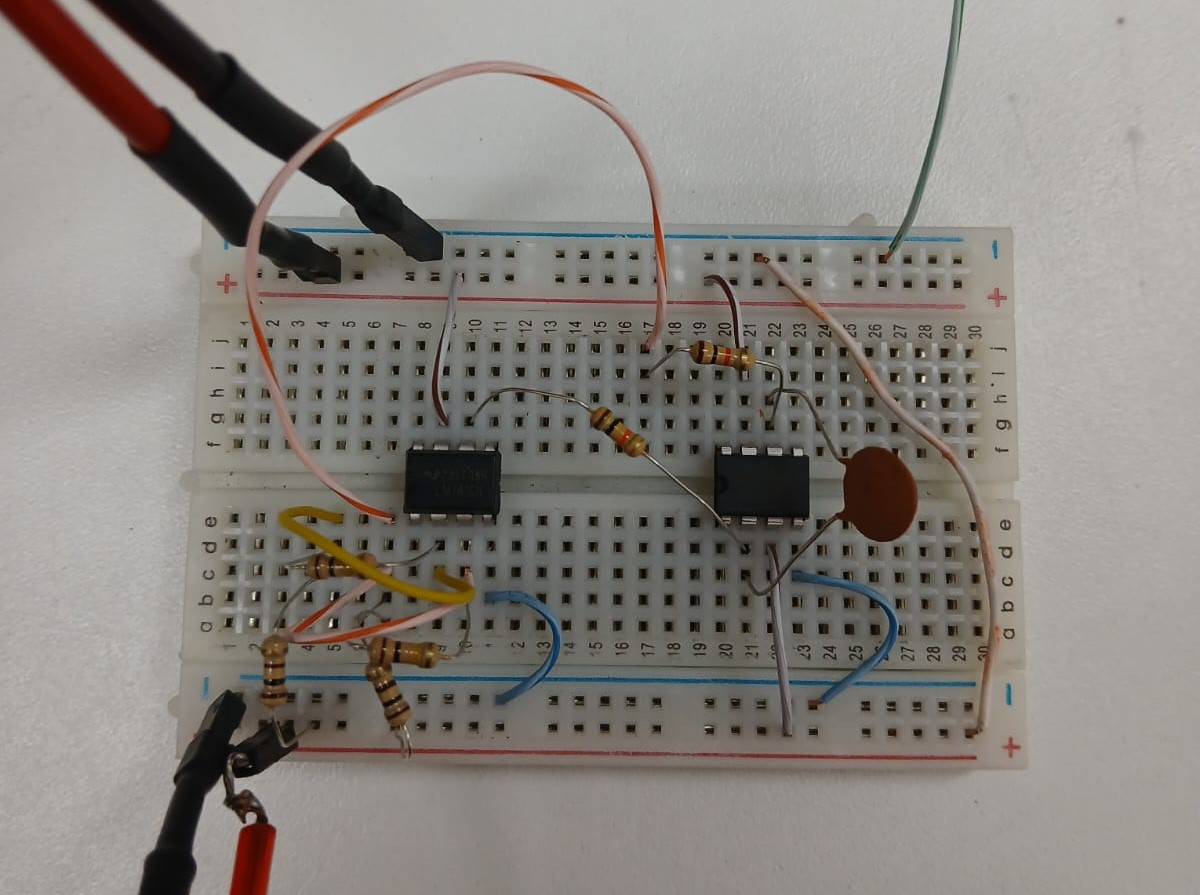
\includegraphics[width=0.4\linewidth]{media/opam-offset}
	\caption{Circuito de prueba para las mediciones offset en los amplificadores operacionales}
	\label{fig:opam-offset}
\end{figure}

Finalmente para resultados obtenidos se debe destacar adicionalmente que $R_6$ tiene una magnitud de 10k $\Omega$.

\section{ Relación entre el $V_{OS}$ y $V_O$}

En un amplificador operacional ideal se tiene la idea de que las corrientes en sus entradas inversora y no-inversora son nulas o equivalentes a 0A, sin embargo de forma experimental y/o real esto no puede ser debido a que los transistores internos requieren la existencia de una corriente de polarización entre sus terminales para que se encuentren en la zona activa; por otro lado al considerar las configuraciones diferenciales estas corrientes de ingreso para cumplir con la paridad considerada en su diseño deberían ser igual, pero a consecuencia de pequeñas variaciones en las entradas o los valores físicos de los propios amplificadores operacionales esto no ocurre existiendo diferencias que afectan a la salida $V_O$ y generando a su vez un voltaje de salida $V_{OS}$ de offset.

Así mismo como se destaca en \ref{eq:vos-calculo} este valor es dependiente del voltaje de salida, la resistencia de retroalimentación y la resistencia en la entrada equivalente a 100 $\Omega$, siendo así la relación matemática se describe entre $V_{OS}$ y $V_{O}$ se define en \ref{eq:vos-demostracion}.

\begin{align}
	V_{OS} = -\frac{ \frac{R_3}{R_3} }{ \frac{R_3}{R_3} + \frac{R_6}{R_3}}*V_O \\
	V_{os} = -\frac{1}{1 + \tfrac{R6}{100}} \cdot V_o \\
	\label{eq:vos-demostracion}
\end{align}

\section{Calculo de $IB^{+}$ en función a $V_O$ y $V_{OS}$}

Para la obtención de la corriente de bias en entrada no-inversora se tuvo en cuenta la tensión de salida $V_O$ con la cual en función a la expresión \ref{eq:ib-plus-vos} y bajo la configuración mostrada en la figura \ref{fig:opam-offset} se estimaron los niveles de tensión y mediante ello el valor de $IB^+$

\begin{equation}
	V_o = -V_{os}\left(1 + \frac{R6}{100}\right) + I_B \cdot R4 \left(1 + \frac{R6}{100}\right)
	\label{eq:ib-plus-vos}
\end{equation}

Los resultados de este procedimiento se muestran en la tabla \ref{tab:valor-bias-noinversora} usando para la misma 2 mediciones de referencia aplicando para ello el multímetro de laboratorioKeithley y uno de referencia Gold Power, obtiendo diferencia no significativas entre las magnitud de voltaje obtenidas con lo cual se puede asegurar cierta precisión en el circuito propuesto.

\begin{table}[]
	\centering
	\begin{tabular}{|l|ll|ll|}
		\hline
		& \multicolumn{2}{c|}{\textbf{Gold   Power}}      & \multicolumn{2}{c|}{\textbf{Keithley}}          \\ \hline
		\textbf{Amp. Operacional} & \multicolumn{1}{l|}{\textbf{Vo}} & \textbf{IB+} & \multicolumn{1}{l|}{\textbf{Vo}} & \textbf{IB+} \\ \hline
		\textbf{LM741}            & \multicolumn{1}{l|}{-10.13}      & -9.0988E-05  & \multicolumn{1}{l|}{-10.172}     & -9.1364E-05  \\ \hline
		\textbf{TL081}            & \multicolumn{1}{l|}{-10.13}      & -9.0988E-05  & \multicolumn{1}{l|}{-10.173}     & -9.1373E-05  \\ \hline
	\end{tabular}
	\caption{Calculo corriente de bias - entrada no-inversora}
	\label{tab:valor-bias-noinversora}
\end{table}

\section{Relación entre $V_O$, $V_{OS}$ e $IB^+$}
Como se menciono previamente la tensión de offset se debe en gran medida a las diferencias entre las corrientes de polarización en la entrada siendo así que existe una relación entre ambos valores y que responden su existencia y demostración en función al principio de superposición, obteniendo así:

\begin{align}
	I_{in} &= I_a + I_B \\
	\frac{0 - V_a}{R_3} &= \frac{V_a - V_o}{R_6} + I_B \\
	-\frac{V_a}{R_3} &= \frac{V_a}{R_6} - \frac{V_o}{R_6} + I_B \\
	V_a \left(\frac{1}{R_3} + \frac{1}{R_6}\right) &= -\frac{V_o}{R_6} + I_B \tag{*} \\	
	I_B &= \frac{V_a - V_{os}}{R_4} \\
	I_B \cdot R_4 + \frac{V_{os}}{R_4} &= V_a \\
	\left(I_B \cdot R_4 + \frac{V_{os}}{R_4}\right)\left(\frac{1}{R_3} + \frac{1}{R_6}\right) &= -V_o \cdot \frac{1}{R_6} + I_B \\
	\left(I_B \cdot R_4 + \frac{V_{os}}{R_4}\right)\left(\frac{R_6}{R_3} + 1\right) &= -V_o + I_B \\ 
	V_o =& -V_{os}\left(\frac{1}{R_3} + \frac{1}{R_6}\right) + I_B \cdot R_4 \left(\frac{1}{R_3} + \frac{1}{R_6}\right) 
	\quad
\end{align}

\section{La expresión de $V_O$ para la obtención de $IB^-$}

Para este caso debido a la relación entre las tensiones de entrada y las corrientes en función \cite{horenstein2000circuitos} la corriente $IB^+$ es igual $IB^-$ pero con el signo o dirección de corriente invertido, por lo que la expresión \ref{eq:valor-ib-inversora} es válida para $IB^-$ considerando el cambio de signo
\begin{equation}
	V_o = V_{os}\left(\frac{1}{R_3} + \frac{1}{R_6}\right) + I_B \cdot R_4 \left(\frac{1}{R_3} + \frac{1}{R_6}\right) 
	\quad
	\label{eq:valor-ib-inversora}
\end{equation}

\section{Corriente de offset $I_{OS}$}

La corriente de offset se toma como el valor medio de las corrientes de polarización (debido al signo) genera un punto intermedio en relación a las magnitudes para cada corriente de entrada.

\begin{align}
	I_{os} &= \frac{I_B^+ - I_B^-}{2} \label{eq:ios} \\
\end{align}

Para el propósito de esta experiencia las mediciones de estas corrientes se tomaron a partir de la formula general, sin embargo una medición mediante las herramientas experimentales sería provechosa para su comprobación y análisis de efectos en las aplicaciones que involucrar amplificadores operacionales.

\section{LM741 y TL081 como DUT (Device Under Test)}

Como se muestra en la figura \ref{fig:opam-offset} el circuito se configuro de forma que sea fácil el intercambio entre los operacionales de test, por lo tanto las mediciones realizadas en cada punto se repitieron para el amplificador operacional de base FET (con el arreglo de resistencias) mostrándose en cada tabla las mediciones realizadas.

\section{Resultados finales}
Del presente informe se puede concluir que:

\begin{itemize}
	\item Se lograron comprobar los diferentes niveles de offset en los amplificadores operacionales, así como la existencia de una desigualdad en las corrientes de polarización generando desviaciones de voltaje en la salida.
	\item A pesar de estas desviaciones se puede inferir que estas se encuentran en la escala de los nA por lo que su efecto puede ser considerado y despreciado en función de la aplicación para los operacionales.
	\item Una verificación más exhaustiva de las corrientes de polarización se puede ejecutar mediante el empleo de instrumentos de medición para corroborar los valores teóricos.
\end{itemize}

























